
\documentclass[10pt,twocolumn,letterpaper]{article}

\usepackage{times}
\usepackage{epsfig}
\usepackage{graphicx}
\usepackage{amsmath}
\usepackage{amssymb}
\usepackage[numbers,sort]{natbib}
%\usepackage[UTF8]{ctex}


\usepackage{subfigure}
\usepackage{upgreek}
\usepackage{multirow}
\usepackage{color}
\usepackage{bm}
\DeclareMathOperator*{\argmin}{arg\,min}
\usepackage{arydshln}
\usepackage{latexsym}

\usepackage{amsthm}
\newtheorem{theorem}{Theorem}
\newtheorem{lemma}[theorem]{Lemma}
\newtheorem{conj}[theorem]{Conjecture}

% Include other packages here, before hyperref.

% If you comment hyperref and then uncomment it, you should delete
% egpaper.aux before re-running latex.  (Or just hit 'q' on the first latex
% run, let it finish, and you should be clear).
\usepackage[pagebackref=true,breaklinks=true,letterpaper=true,colorlinks,bookmarks=false]{hyperref}




\begin{document}

%%%%%%%%% TITLE
\title{A Realistic Dataset for Image Denoising and Demosaicking}

\maketitle



%%%%%%%%% ABSTRACT
\begin{abstract}
In this report, we introduce the motivation, idea, procedure, and results of our real noisy image dataset with ``ground truth''. In this paper, we propose to simultaneously employing the spatial and temporal information to construct a real-world dataset which contain the original raw images as well as corresponding ``ground truth'' images. This dataset can be used in real world image denoising, demosaicking, and joint denoising and demosaicking (JDD) problems.
\end{abstract}

%%%%%%%%% BODY TEXT
\section{Introduction}

According to \cite{healey1994radiometric}, the noise corrupted in the imaging process is signal dependent and comes from five main sources:\ photon shot, fixed pattern, dark current, readout, and quantization noise. The noise model could be approximatedly modeled as 
\begin{equation}
\bm{P} = f((g_{cv}(\bm{C}+\bm{D})+\bm{N}_{reset})g_{out}+\bm{N}_{out})+\bm{Q}
\end{equation}


Nam et al. \cite{crosschannel2016} constructed a realistic dataset including real noisy images and correpsonding ``ground truth''. This dataset includes noisy images of 11 static scenes.\ The noisy images were collected under controlled indoor environment.\ Each scene was shot 500 times under the same camera and camera setting.\ The mean image of the 500 shots is roughly taken as the ``ground truth''. Khashabi et al. \cite{khashabi2014joint} constructed a realistic dataset including CFA images and corresponding sRGB images. Each image is sub-sampled to reduce the influence of the noise.

\section{Motivation}

Although this dataset could be roughly used for realistic image denoising, it has many key problems:

\textbf{Problem 1}:The noise in sRGB space is no longer independent with the noise on other pixels, which only holds in the raw space. Thus, averaging the pixels on sRGB space is not reasonable. 

\textbf{Problem 2}: Capturing 500 images take a long time, during which the scene should hasno change in lighting conditions. So We cannot capturing natural scenes or human which would be almost static in a short time while changing during a long time. For example, we need 500 seconds to take 500 images with a normal camera. 

\textbf{Problem 3}: Take 500 images may generate shift on the spatial dimension.

\textbf{Problem 4}: The huge amount of heat generated by continuous taking photos  will make the noise bigger

\textbf{Problem 5}: The physical property of each pixel has built-in attributes which make the noise in that pixel has a built-in tendency which cannot be averaged out by only using the 500 samples on that pixel.

\textbf{Problem 6}: Some special cameras, such as the camera in DJI UAVs, can only capure about 10 images each time and will automatically change the parameters in the next capturing. Hence, we cannot guarantee that the 500 images share the same camera settings.

\textbf{Problem 7}: The images in \cite{khashabi2014joint} are too small (of size $200\times 200$) to contain any detailed information which can reflect the effectiveness of the demosaicking methods.


\section{Idea: Combining Spatial and Temporal Information}

The above 6 problems are the major problems we need to solve if we want to take 500 pictures for each scene. The solution to \textbf{Problem 1} is very simple, we need to average the captured pictures in the raw space other the sRGB space. To solve the \textbf{Problems 2-7}, we can take few (e.g., 10) pictures instead of 500. To make up the decreasing of the temporal information, we can make use of the spatial information. That is, we can first average each CFA image via sub-sampling on the spatial direction and then average the 10 images along the temporal direction.


In Figure \ref{f1}, we average the pixels of the $W\times W$ patch to form a red pixel, and average the pixels in the right $W\times W$ patch to form a green pixel, and average the pixels in the below $W\times W$ patch to form another green pixel, and average the pixels in the lower right $W\times W$ patch to form another blue pixel. The other patches are performed in a similar way. 

\begin{figure}
\centering
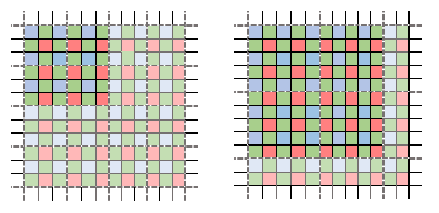
\includegraphics[width=0.95\linewidth]{CFA.png}
\caption{Averaging with odd windows, with $W = 1$ (left) and $W = 2$ (right),
where the window size is $(2W + 1)\times (2W + 1)$.
}
\label{f1}
\end{figure}


\section{Preliminary Results}
We design a camera pipeline which includes (in sequential order)
\begin{itemize}
\item Black Light Subtraction;
\item Spatial Sub-sampling; 
\item Temporal Averaging (10 images);
\item White Balance;
\item Demosaicking;
\item Color Space Transfer;
\item Gamma Correction;
\end{itemize}

The following example (Figure \ref{f2} and \ref{f3}) is given by Hui Li. The Figure \ref{f2} is the sRGB image captured by the camera SONY A7 II when ISO=800. The Figure \ref{f3} is obtained by processing the original raw image without Color Space Transfer. The Demosaicking step is performed via the Deep Residual Network.

The following example (Figures \ref{f4} and \ref{f5}) is given by Jun Xu. The 
Figure \ref{f4} is the sRGB image processed by the raw image captured by the camera SONY A7 II when ISO=12800. The Figure \ref{f5} is obtained by processing the original raw image with a simple camera pipeline.

One can see from the two examples that the noise in the raw images can be highly reduced. However, in some dark area, there still exists some color artifacts or noise. 

\section{Limitation of the Proposed Method}
There are two major limitations:
\begin{itemize}
\item In some dark area, there still exists some color artifacts or noise. I think these problems can hardly be solved by adding more frames. 
\item The quality of the image generated by our pipeline is limited. This is because the pipeline is simple and rough. 
\end{itemize}

\section{Furure Work}

I think we can perform spatial sub-sampling and temporal averaging directly on sRGB images captured by cameras. In this way, we can construct ``ground truth'' images both for real image denoising and demosaicking problems.


\begin{figure*}
\centering
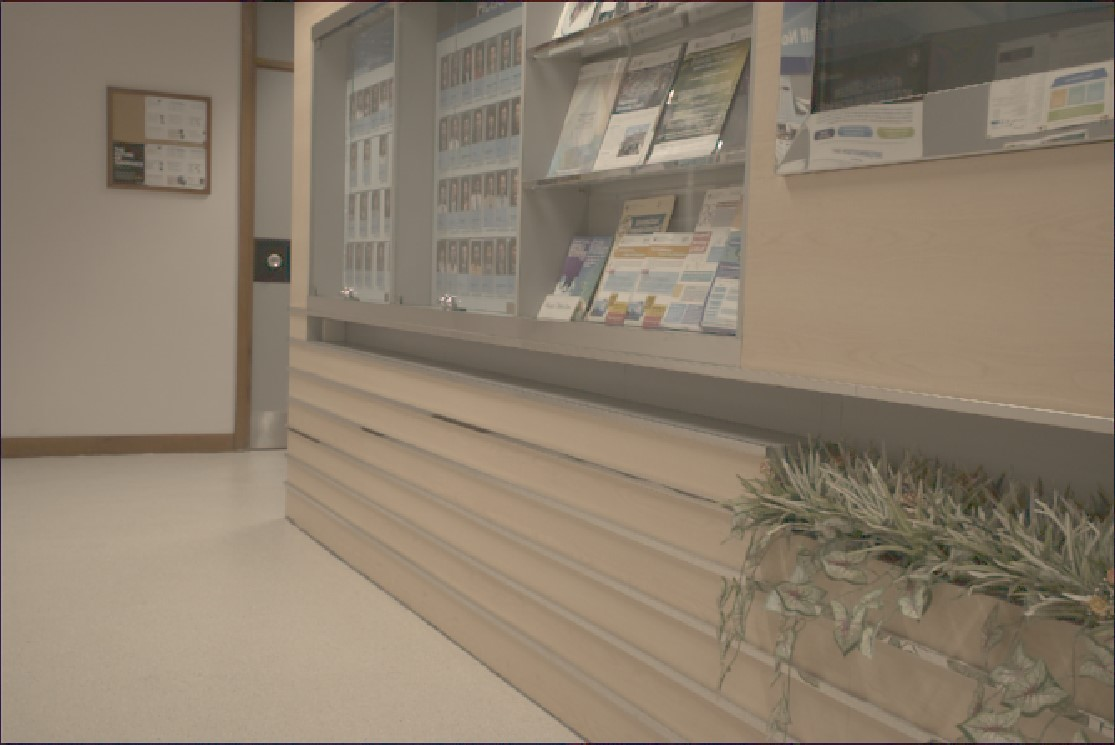
\includegraphics[width=0.8\linewidth]{resize_DSC01764.JPG}
\vspace{-4mm}
\caption{The real noisy image processed by the raw image captured by SONY A7 II when ISO=800.
}
\label{f2}
\end{figure*}


\begin{figure*}
\centering
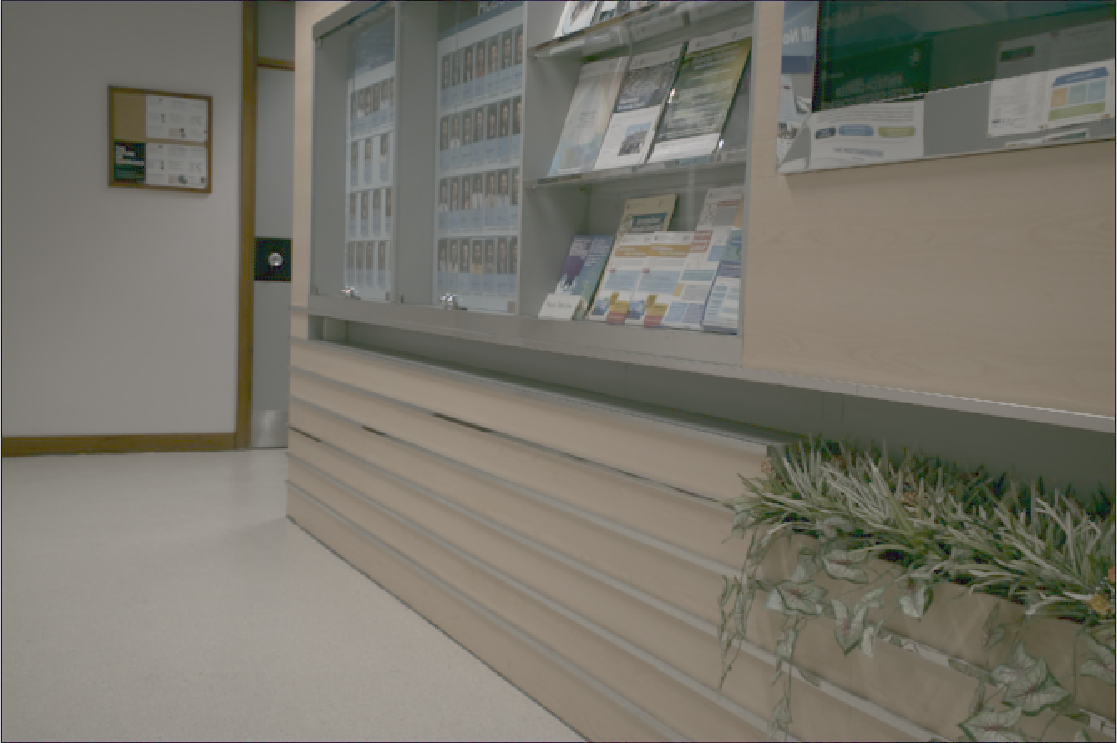
\includegraphics[width=0.8\linewidth]{STA.png}
\vspace{-4mm}
\caption{The averaged image obtained by spatial sub-sampling and temporal averaging.
}
\label{f3}
\end{figure*}


\begin{figure*}
\centering
\includegraphics[width=0.8\linewidth]{resize_DSC01814_5BrightGammaCorrected.png}
\vspace{-4mm}
\caption{The real noisy image processed by the raw image captured by SONY A7 II when ISO=12800.
}
\label{f4}
\end{figure*}


\begin{figure*}
\centering
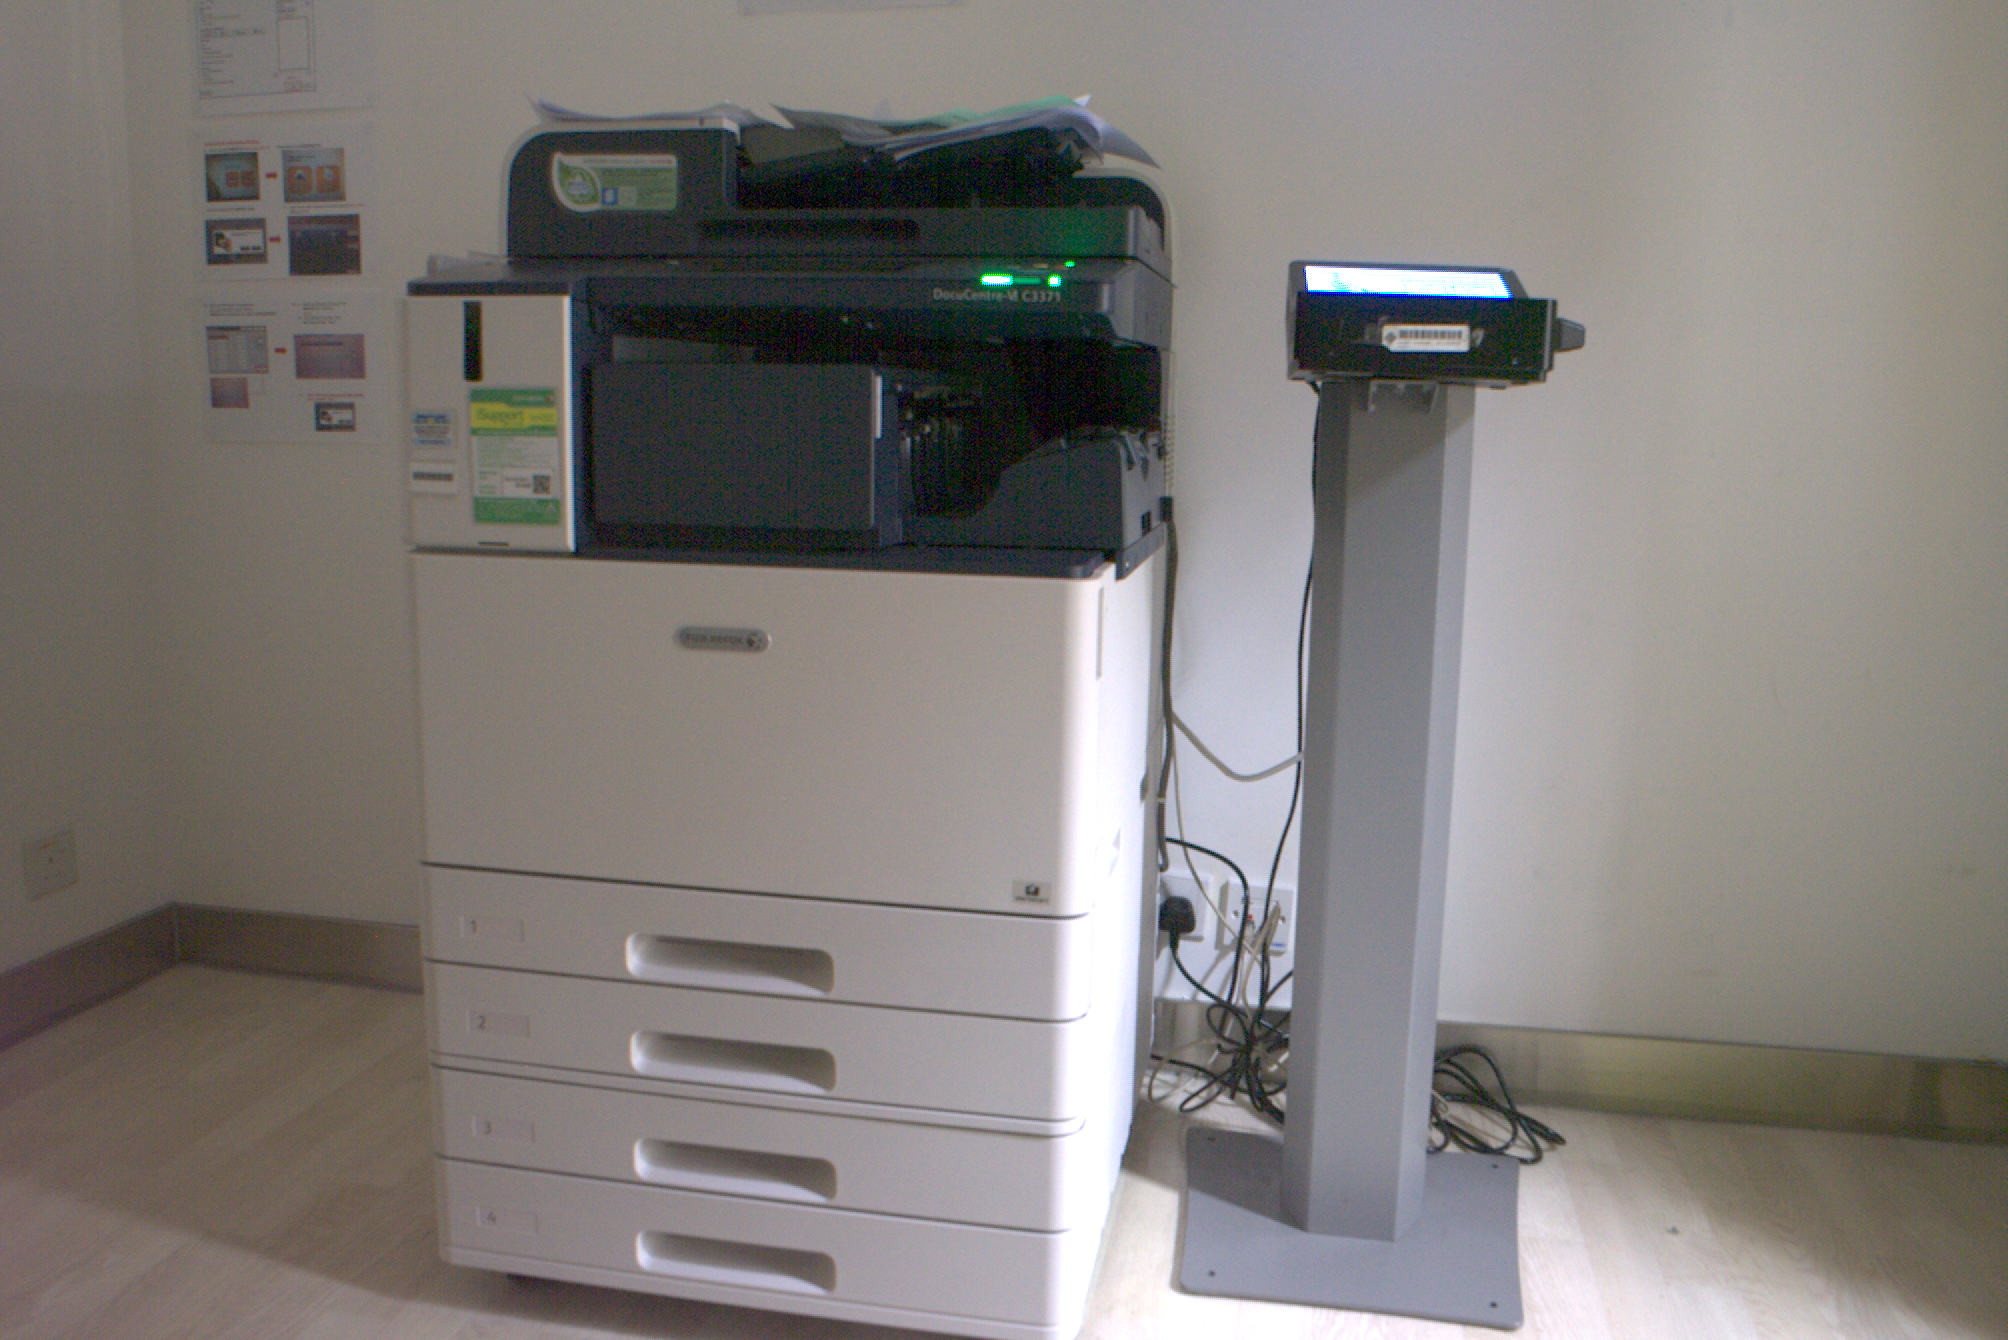
\includegraphics[width=0.8\linewidth]{SONY_A7II_ISO12800_A_5BrightGammaCorrected.png}
\vspace{-4mm}
\caption{The averaged image obtained by spatial sub-sampling and temporal averaging.
}
\label{f5}
\end{figure*}


{
\small
\bibliographystyle{unsrt}
\bibliography{egbib}
}

\end{document}
